% Guía de lectura de los planos v2.0 del brazo XK-JS1-1 (P&ID-B4G-01 y E-B4G-01).
% Las imágenes de img/ las genera recortes.py desde los PDF públicos de documentacion/planos_isa/.
\documentclass[11pt]{article}
% Estilo común de los manuales del gemelo digital (se incluye con \input)
\usepackage{geometry}
\geometry{letterpaper, margin=2.2cm}
\usepackage[spanish, es-nodecimaldot, mexico]{babel}
\usepackage[utf8]{inputenc}
\usepackage[T1]{fontenc}
\usepackage{lmodern}
\usepackage{amsmath,amssymb}
\usepackage[table]{xcolor}
\definecolor{naranja}{RGB}{194,98,12}
\definecolor{rojo}{RGB}{192,57,43}
\definecolor{verde}{RGB}{30,120,70}
\definecolor{azulw}{RGB}{0,103,184}
\definecolor{azulg}{RGB}{70,90,120}
\definecolor{gris}{RGB}{242,242,242}
\definecolor{grisos}{RGB}{90,90,90}
\usepackage{booktabs,longtable,array,tabularx}
\usepackage{graphicx}
\usepackage{float}
\usepackage{caption}
\captionsetup{font=small, labelfont=bf}
\usepackage{tikz}
\usetikzlibrary{positioning,arrows.meta,fit,calc,shapes.geometric,decorations.pathreplacing,backgrounds}
\usepackage{enumitem}
\setlist{itemsep=2pt}
\usepackage{listings}
\lstset{basicstyle=\ttfamily\small, frame=single, backgroundcolor=\color{gris}, breaklines=true,
  columns=fullflexible, keepspaces=true, extendedchars=true, upquote=true,
  literate={á}{{\'a}}1 {é}{{\'e}}1 {í}{{\'i}}1 {ó}{{\'o}}1 {ú}{{\'u}}1 {ñ}{{\~n}}1 {Á}{{\'A}}1 {É}{{\'E}}1
           {Í}{{\'I}}1 {Ó}{{\'O}}1 {Ú}{{\'U}}1 {Ñ}{{\~N}}1 {ü}{{\"u}}1 {¿}{{?`}}1 {¡}{{!`}}1 {…}{{...}}3
           {θ}{{$\theta$}}1 {·}{{$\cdot$}}1 {«}{{\guillemotleft}}1 {»}{{\guillemotright}}1 {°}{{$^\circ$}}1}
\usepackage{hyperref}
\hypersetup{colorlinks=true, linkcolor=naranja, urlcolor=naranja}
\usepackage{fancyhdr}
\pagestyle{fancy}
\fancyhf{}
\cfoot{\small \thepage}
\newcommand{\codigo}[1]{\texttt{#1}}
\newcommand{\archivo}[1]{\textbf{\texttt{#1}}}
\newcommand{\aviso}[1]{\par\smallskip\noindent\colorbox{rojo!10}{\parbox{\dimexpr\linewidth-2\fboxsep}{\textbf{\color{rojo}Atención.} #1}}\par\smallskip}
\newcommand{\nota}[1]{\par\smallskip\noindent\colorbox{gris}{\parbox{\dimexpr\linewidth-2\fboxsep}{#1}}\par\smallskip}
\tikzset{
  marca/.style={circle, fill=naranja, text=white, font=\bfseries\footnotesize, inner sep=1.4pt, minimum size=4.6mm, draw=white, line width=0.8pt},
  caja/.style={draw, rounded corners=2pt, fill=gris, align=center, font=\small, minimum height=10mm, inner sep=4pt},
  cajab/.style={caja, fill=white},
  cajan/.style={caja, fill=naranja!14, draw=naranja!70!black},
  paso/.style={draw, rounded corners=2pt, fill=white, align=left, font=\small, text width=3.4cm, minimum height=15mm, inner sep=5pt},
  num/.style={circle, fill=naranja, text=white, font=\bfseries\small, inner sep=1.5pt, minimum size=6mm},
  flecha/.style={-{Stealth[length=2.2mm]}, thick},
  dflecha/.style={{Stealth[length=2.2mm]}-{Stealth[length=2.2mm]}, thick},
  etiq/.style={font=\scriptsize, align=center},
}
\DeclareRobustCommand{\num}[1]{\tikz[baseline=-0.7ex]\node[marca]{#1};}
% \captura{ancho}{archivo}{marcas en coordenadas 0-1 desde la esquina inferior izquierda}
\newcommand{\captura}[3]{%
  \begin{tikzpicture}
  \node[anchor=south west, inner sep=0, draw=black!25] (img) {\includegraphics[width=#1]{#2}};
  \begin{scope}[x={(img.south east)}, y={(img.north west)}]
  #3
  \end{scope}
  \end{tikzpicture}}
% ventana dibujada (consolas y diálogos): \ventana{ancho}{alto}{título}{contenido}
\newcommand{\ventana}[4]{%
\begin{tikzpicture}
\node[draw=black!50, fill=white, minimum width=#1, minimum height=#2, anchor=north west, inner sep=0] (v) at (0,0) {};
\fill[black!8] (v.north west) rectangle ($(v.north east)+(0,-6mm)$);
\node[anchor=west, font=\scriptsize] at ($(v.north west)+(2mm,-3mm)$) {#3};
\node[anchor=east, font=\scriptsize] at ($(v.north east)+(-2mm,-3mm)$) {--\quad$\square$\quad$\times$};
\node[anchor=north west, inner sep=3mm, text width=#1-6mm, font=\scriptsize\ttfamily, align=left] at ($(v.north west)+(0,-6mm)$) {#4};
\end{tikzpicture}}

\graphicspath{{img/}}
\setlength{\headheight}{14pt}
\lhead{\small Brazo XK-JS1-1 · Guía de lectura de los planos}
\rhead{\small UMSA · II/2026}
\renewcommand{\headrulewidth}{0.4pt}
\newcommand{\zona}[1]{\textsf{\small[#1]}}
\newcommand{\fig}[3][\linewidth]{\begin{figure}[H]\centering\includegraphics[width=#1]{#2}\caption{#3}\end{figure}}
\newcommand{\clave}[1]{\par\smallskip\noindent\colorbox{verde!10}{\parbox{\dimexpr\linewidth-2\fboxsep}{\textbf{\color{verde}Idea clave.} #1}}\par\smallskip}
\tikzset{
  bloque/.style={draw, rounded corners=2pt, fill=white, align=center, font=\small, minimum height=10mm, inner sep=4pt, text width=#1},
  bloque/.default=26mm,
  hilo/.style={line width=0.9pt},
  hpos/.style={hilo, rojo},
  neg/.style={hilo, azulw},
  sen/.style={hilo, verde},
}

\begin{document}
\begin{titlepage}
\centering
\vspace*{0.6cm}
{\large Universidad Mayor de San Andrés · Facultad de Ingeniería\par}
{\large Carrera de Ingeniería Electrónica\par}
\vspace{0.8cm}
{\color{naranja!80!black}\rule{\linewidth}{1.5pt}\par}
\vspace{0.3cm}
{\Large Guía de lectura de los planos v2.0\par}
\vspace{0.2cm}
{\huge\bfseries Diagrama P\&ID y esquema eléctrico del brazo de 4 GDL\par}
\vspace{0.3cm}
{\color{naranja!80!black}\rule{\linewidth}{1.5pt}\par}
\vspace{0.6cm}
{\large P\&ID-B4G-01 (ISA-5.1-2009) · E-B4G-01 hojas 1 y 2 (IEC 60617 / IEC 60204-1)\par}
\vspace{0.8cm}
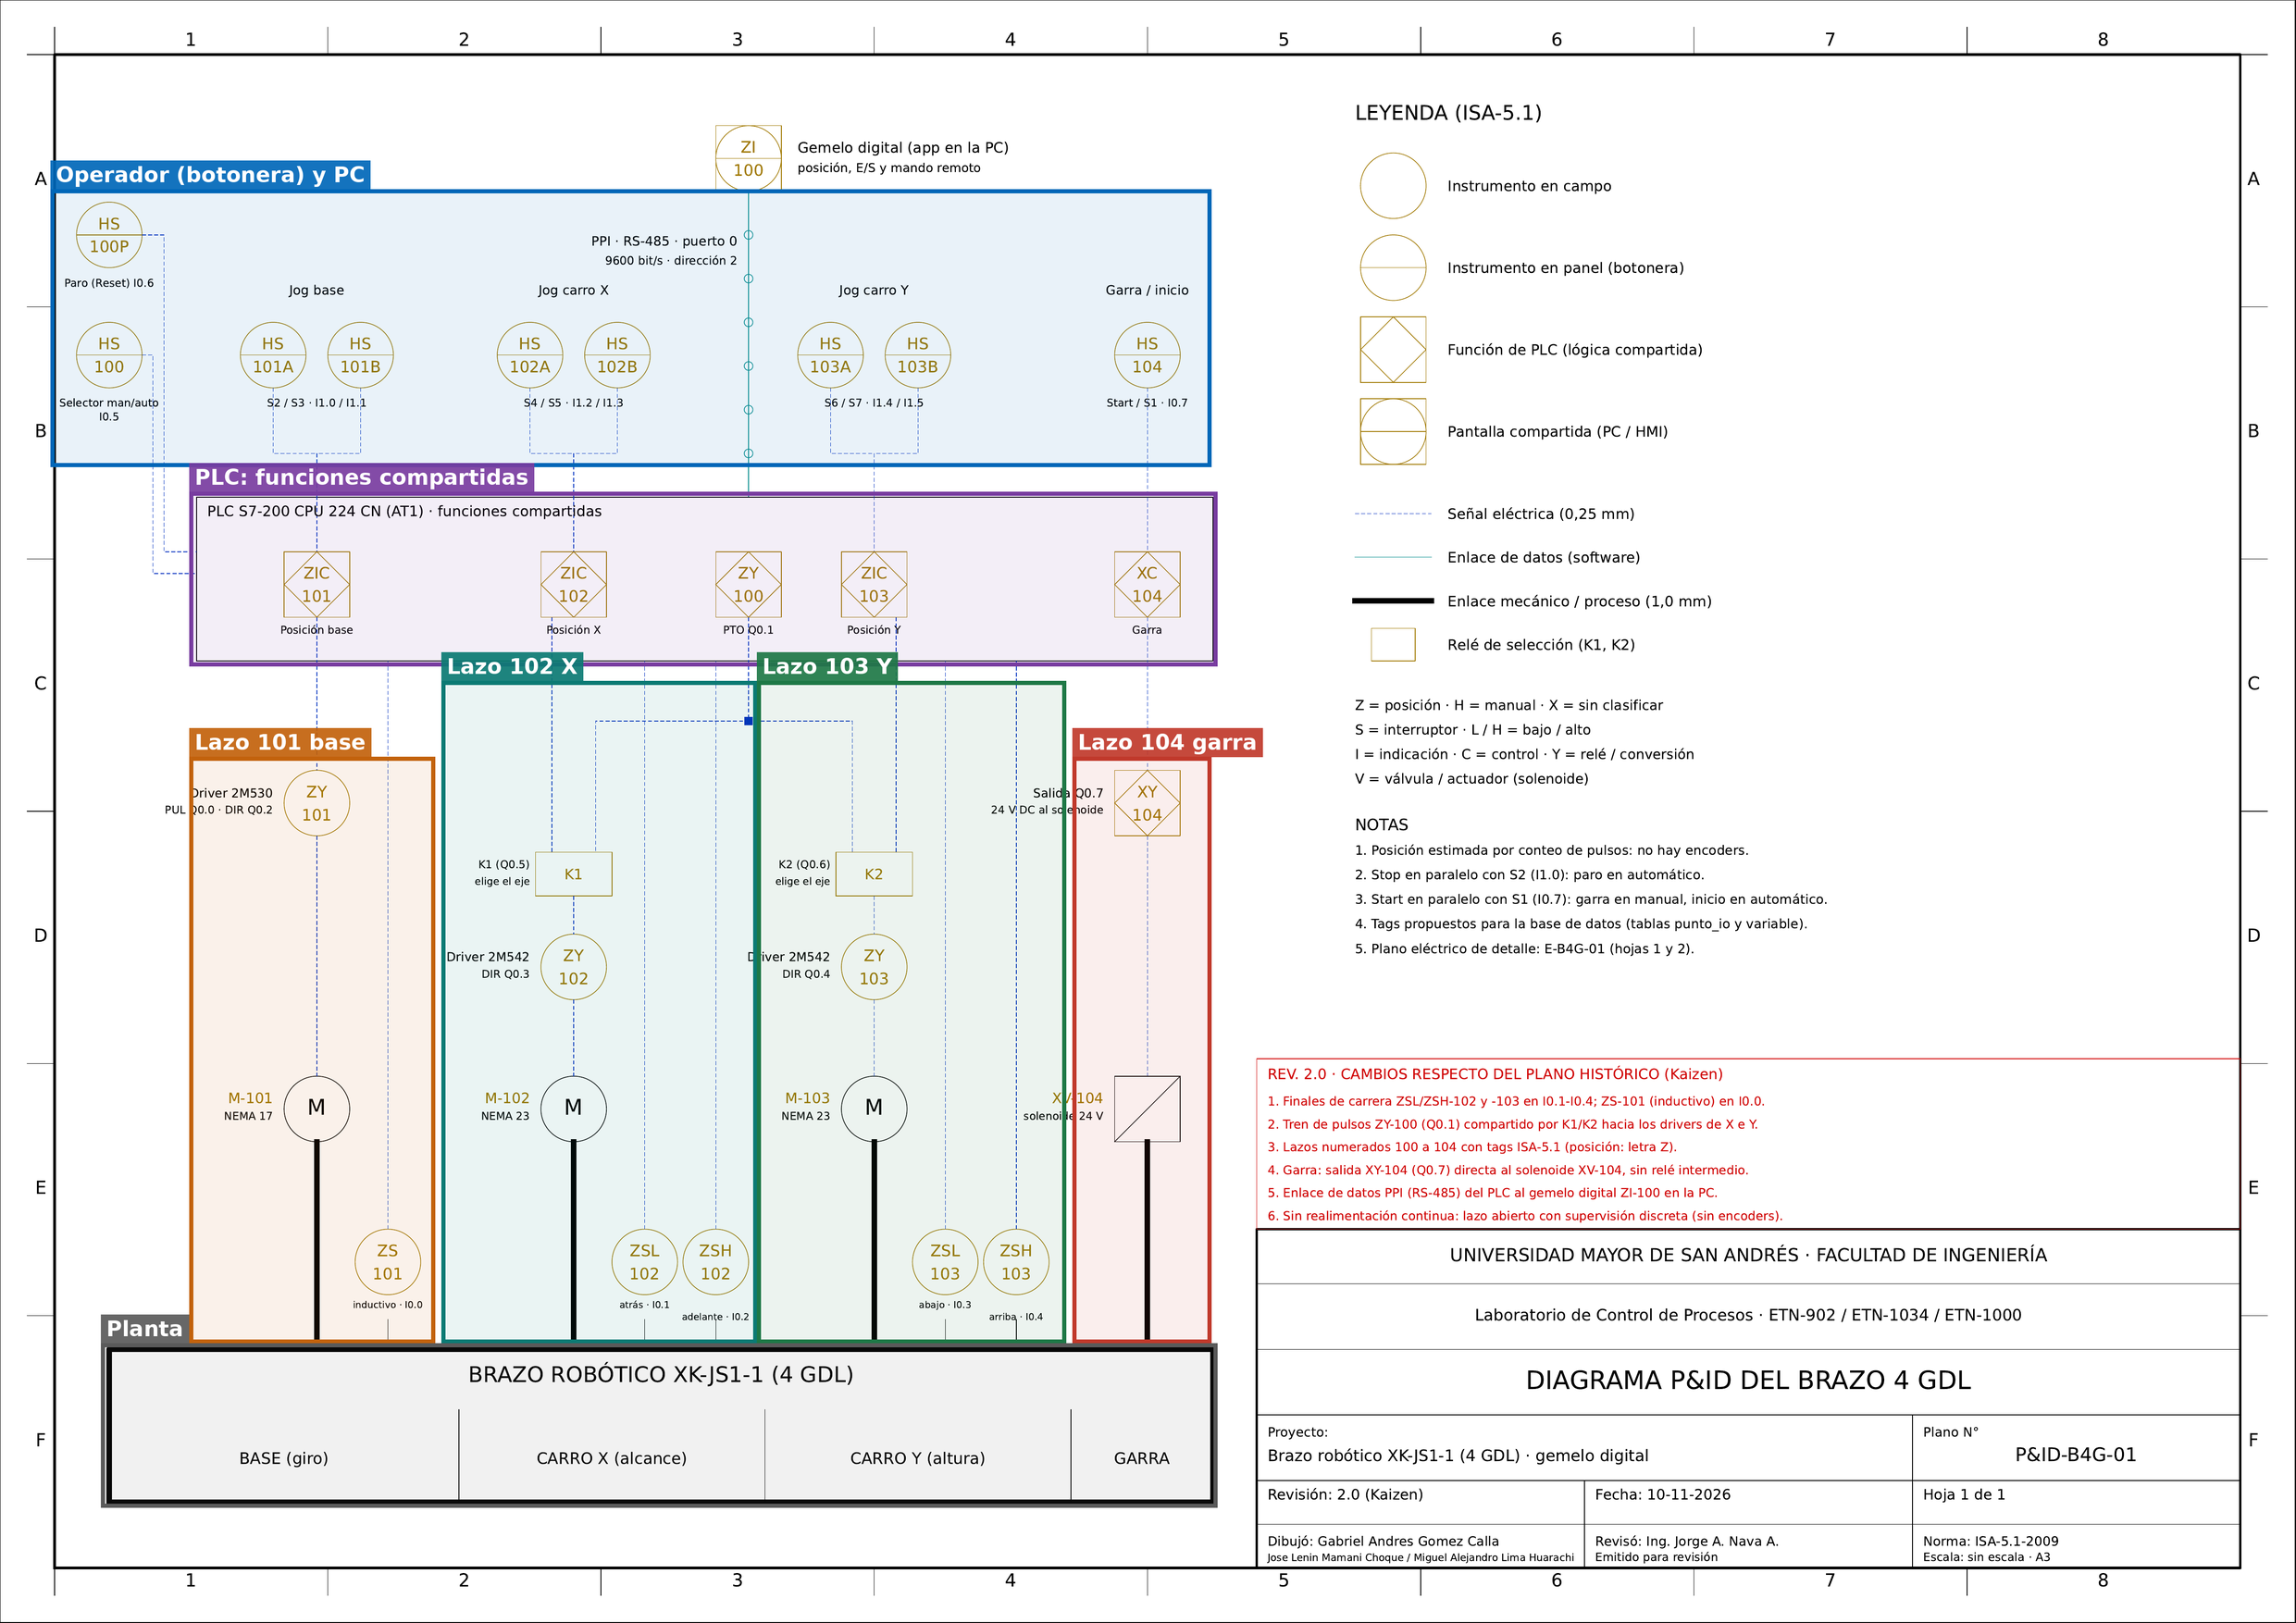
\includegraphics[width=0.82\linewidth]{pid_completo}
\vfill
{\large Planta: brazo robótico XK-JS1-1 · Fase I: ingeniería inversa y auditoría Kaizen\par}
\vspace{0.2cm}
{\small ETN-902 · ETN-1034 · ETN-1000 · Escuadra del brazo de 4 GDL · La Paz, II/2026\par}
\end{titlepage}

\tableofcontents
\newpage

\section{Para qué sirve esta guía}
La escuadra levantó el brazo XK-JS1-1 por ingeniería inversa y redibujó sus dos planos en la versión 2.0 (Kaizen):
\begin{itemize}
\item el \textbf{diagrama P\&ID} (plano P\&ID-B4G-01), que dice \emph{qué} hace cada elemento: qué mide, qué controla y qué acciona;
\item el \textbf{esquema eléctrico} (plano E-B4G-01), que dice \emph{cómo} está cableado: hoja 1 de potencia y hoja 2 de mando con el PLC.
\end{itemize}
Esta guía recorre los dos planos zona por zona con recortes ampliados, explica cada símbolo y sigue una señal de punta a punta. Al final lista lo que se corrigió frente a los planos históricos y las mejoras propuestas.

\nota{\textbf{Cómo citar una zona.} Los planos son A3 con un marco de referencias: columnas 1 a 8 y filas A a F. En esta guía, \zona{C3} significa fila C, columna 3. En el esquema eléctrico, una referencia como \codigo{/2.1} significa \emph{hoja 2, columna 1}: indica dónde continúa un cable o dónde está dibujado el contacto de un relé.}

\nota{\textbf{Origen de los datos.} Todo lo que dice esta guía sale de los planos v2.0, de las placas de los equipos, de las fotos del tablero y de las pruebas con el PLC en marcha.}

\subsection{La planta en un solo diagrama}
Antes de entrar en los planos conviene tener la cadena completa en la cabeza. Todo el brazo funciona así:

\begin{figure}[H]\centering
\begin{tikzpicture}[x=1cm,y=1cm]
\node[bloque=25mm, fill=azulw!8] (op) at (0,1.3) {Operador\\\scriptsize botonera (HS)};
\node[bloque=25mm, fill=azulw!8] (pc) at (0,-1.3) {PC\\\scriptsize gemelo digital ZI-100};
\node[bloque=25mm, fill=naranja!12] (plc) at (3.9,0) {PLC S7-200\\CPU 224\\\scriptsize lógica ZIC / XC};
\node[bloque=27mm] (drv) at (8,1.3) {Drivers\\2M542 / 2M530\\\scriptsize ZY-101/102/103};
\node[bloque=27mm, fill=naranja!6] (rel) at (8,-1.3) {Salida Q0.7\\\scriptsize XY-104, 24 V DC};
\node[bloque=25mm] (mot) at (12,1.3) {Motores\\paso a paso\\\scriptsize M-101/102/103};
\node[bloque=25mm] (sol) at (12,-1.3) {Solenoide\\\scriptsize XV-104};
\node[bloque=25mm, fill=gris] (br) at (12,-4) {\textbf{Brazo}\\\scriptsize base, carros X e Y, garra};
\node[bloque=27mm, fill=verde!10] (sw) at (8,-4) {Sensores\\\scriptsize ZS-101 inductivo\\ZSL / ZSH finales};
\draw[flecha] (op) -- (plc);
\draw[flecha, azulw, dashed] (pc) -- node[etiq, below right]{PPI RS-485} (plc);
\draw[flecha] (plc) -- node[etiq, above left]{pulsos y dir.} (drv);
\draw[flecha] (plc) -- node[etiq, below left]{XC-104} (rel);
\draw[flecha] (drv) -- (mot);
\draw[flecha] (rel) -- (sol);
\draw[line width=2pt] (mot.east) -- ++(0.5,0) |- (br.east);
\draw[line width=2pt] (sol) -- (br);
\draw[flecha] (br) -- node[etiq, above]{detectan} (sw);
\draw[flecha, verde] (sw.west) -| node[etiq, pos=0.3, above]{I0.0 a I0.4} (plc.south);
\end{tikzpicture}
\caption{Cadena de mando del brazo. Las flechas gruesas son enlaces mecánicos; la discontinua es el enlace de datos con la PC.}
\end{figure}

\clave{El brazo trabaja en \textbf{lazo abierto}. No hay encoders: el PLC no mide la posición, la \emph{estima} contando los pulsos que manda a cada driver. Los sensores solo dicen ``llegué al origen'' o ``llegué al extremo''. Si un motor pierde pasos, el PLC no se entera hasta el próximo homing.}

%======================================================================
\section{Diagrama P\&ID (plano P\&ID-B4G-01)}
%======================================================================
\fig{pid_completo}{Plano P\&ID completo con sus zonas marcadas: operador y PC arriba, PLC en el medio, un lazo por eje y la planta abajo. A la derecha están la leyenda, las notas, los cambios de la revisión 2.0 y el cajetín.}

El P\&ID se lee \textbf{de arriba hacia abajo}, en el mismo orden en que viaja una orden: el operador o la PC dan la orden, el PLC la procesa, los drivers y relés la convierten en potencia, los motores mueven el brazo y los sensores devuelven la información al PLC. Cada columna vertical es un \textbf{lazo} (un eje) y todo lo que tiene el mismo número pertenece al mismo lazo.

\subsection{La leyenda: los cuatro tipos de globo}
\begin{figure}[H]\centering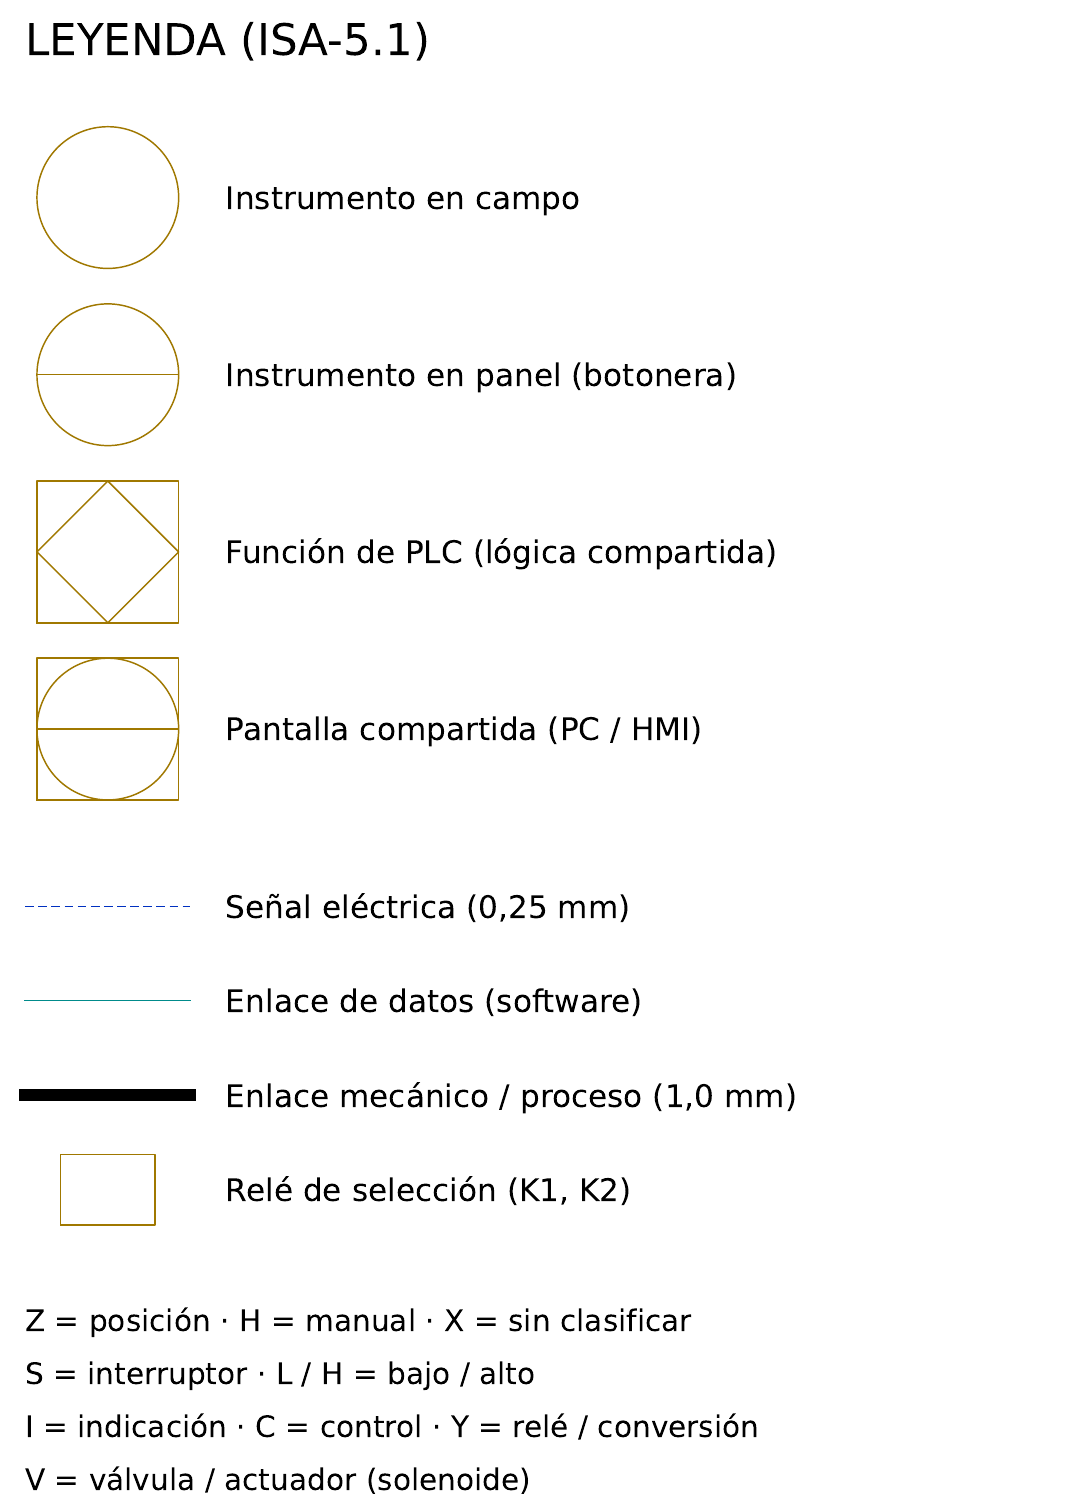
\includegraphics[width=0.65\linewidth, height=8.5cm, keepaspectratio]{pid_leyenda}\end{figure}
La norma ISA-5.1 usa la \emph{forma} del símbolo para decir \emph{dónde está} el instrumento y \emph{qué tipo} de cosa es \zona{A6--C6}:
\begin{itemize}
\item \textbf{Círculo simple:} instrumento \emph{en campo}, montado en la máquina. Ejemplos: el sensor inductivo ZS-101 y los finales de carrera.
\item \textbf{Círculo con una línea horizontal:} instrumento \emph{en el panel}, accesible al operador. Son los pulsadores y el selector de la botonera (HS).
\item \textbf{Rombo dentro de un cuadrado:} \emph{función de PLC}. No es un aparato físico, es una parte del programa (lógica compartida). Ejemplos: ZIC-101 y XC-104.
\item \textbf{Círculo dentro de un cuadrado:} \emph{pantalla compartida}, es decir, una vista en una PC o HMI. Es el gemelo digital ZI-100.
\end{itemize}
Las líneas también tienen significado:
\begin{itemize}
\item \textbf{Discontinua fina (0,25 mm):} señal eléctrica, un cable.
\item \textbf{Continua fina:} enlace de datos por software (comunicación).
\item \textbf{Continua gruesa (1,0 mm):} enlace mecánico; el motor mueve físicamente el eje.
\end{itemize}
El rectángulo pequeño es un \textbf{relé de selección} (K1 y K2).

\subsection{Cómo se lee un tag}
Cada globo lleva arriba unas letras y abajo un número. Por ejemplo \textbf{ZSL-102}:

\begin{center}
\begin{tikzpicture}
\node[circle, draw=naranja!80!black, thick, minimum size=17mm, align=center, font=\large\color{naranja!80!black}] (g) {ZSL\\[-1mm]\rule{12mm}{0pt}\\[-3mm]102};
\draw[naranja!80!black] ($(g.west)+(0,0.0)$) -- ($(g.east)+(0,0.0)$);
\node[right=14mm of g, yshift=9mm, align=left, font=\small] (a) {\textbf{Z} = variable medida: \textbf{posición}};
\node[right=14mm of g, yshift=2mm, align=left, font=\small] (b) {\textbf{S} = función: \textbf{interruptor} (switch)};
\node[right=14mm of g, yshift=-5mm, align=left, font=\small] (c) {\textbf{L} = modificador: \textbf{bajo} (low), el extremo de origen};
\node[right=14mm of g, yshift=-12mm, align=left, font=\small] (d) {\textbf{102} = número de lazo: \textbf{carro X}};
\draw[-{Stealth}, grisos] ($(g.north)+(-2mm,-5mm)$) -- (a.west);
\draw[-{Stealth}, grisos] ($(g.north)+(0mm,-5mm)$) -- (b.west);
\draw[-{Stealth}, grisos] ($(g.north)+(3mm,-5mm)$) -- (c.west);
\draw[-{Stealth}, grisos] ($(g.south)+(0,4mm)$) -- (d.west);
\end{tikzpicture}
\end{center}

\begin{center}\small
\begin{tabularx}{\linewidth}{c >{\raggedright}X c >{\raggedright\arraybackslash}X}
\toprule
\multicolumn{2}{c}{\textbf{Primera letra (variable)}} & \multicolumn{2}{c}{\textbf{Letras siguientes (función)}}\\
\midrule
Z & posición (de los ejes) & S & interruptor (switch)\\
H & manual (hand): lo acciona una persona & I & indicación (muestra un valor)\\
X & sin clasificar (se usa para la garra) & C & control (decide)\\
 & & Y & relé, conversión o cálculo\\
 & & V & válvula o actuador (el solenoide)\\
 & & L / H & bajo / alto (los dos extremos)\\
\bottomrule
\end{tabularx}\end{center}

Así, \textbf{HS} es un interruptor manual (un pulsador), \textbf{ZIC} un controlador indicador de posición, \textbf{ZY} un relé o conversor de posición (el driver convierte pulsos en corriente para el motor), \textbf{XY} el relé de la garra y \textbf{XV} su actuador.

\subsection{Los cinco lazos}
\begin{center}\small
\begin{tabularx}{\linewidth}{c >{\raggedright}p{2.3cm} >{\raggedright\arraybackslash}X}
\toprule \textbf{Lazo} & \textbf{Eje} & \textbf{Elementos}\\ \midrule
100 & Común & HS-100 selector manual/automático (I0.5) · HS-100P paro/reset (I0.6) · ZY-100 tren de pulsos compartido (Q0.1) · ZI-100 gemelo digital\\
101 & Base (giro) & HS-101A/B jog (I1.0/I1.1) · ZIC-101 · ZY-101 driver 2M530 · M-101 NEMA 17 · ZS-101 inductivo (I0.0)\\
102 & Carro X (alcance) & HS-102A/B jog (I1.2/I1.3) · ZIC-102 · K1 (Q0.5) · ZY-102 driver 2M542 · M-102 NEMA 23 · ZSL-102 atrás (I0.1) · ZSH-102 adelante (I0.2)\\
103 & Carro Y (altura) & HS-103A/B jog (I1.4/I1.5) · ZIC-103 · K2 (Q0.6) · ZY-103 driver 2M542 · M-103 NEMA 23 · ZSL-103 abajo (I0.3) · ZSH-103 arriba (I0.4)\\
104 & Garra & HS-104 Start/S1 (I0.7) · XC-104 lógica · XY-104 salida Q0.7 · XV-104 solenoide 24 V\\
\bottomrule\end{tabularx}\end{center}
Los mismos tags están en la base de datos (tablas \codigo{punto\_io} y \codigo{variable}): el plano, el programa del PLC y la base de datos llaman igual a cada señal. Esa es la \textbf{trazabilidad ISA} del laboratorio III.

\subsection{Zona del operador y de la PC \zona{A1--B5}}
\fig{pid_operador}{Botonera del operador (globos con línea: instrumentos en panel) y gemelo digital ZI-100 conectado por PPI.}
\begin{itemize}
\item \textbf{HS-100P} (I0.6): paro o reset. \textbf{HS-100} (I0.5): selector manual/automático. Sus líneas discontinuas bajan por la izquierda y entran al recuadro del PLC.
\item \textbf{Jog} de cada eje: dos pulsadores por eje, A y B, uno por sentido. Base HS-101A/B (I1.0/I1.1), carro X HS-102A/B (I1.2/I1.3) y carro Y HS-103A/B (I1.4/I1.5). Debajo de cada par se lee el nombre del pulsador en el tablero (S2 a S7) y su entrada.
\item \textbf{HS-104} (I0.7): Start / S1. En manual abre o cierra la garra; en automático arranca la secuencia.
\item \textbf{ZI-100}, gemelo digital: la aplicación en la PC que muestra la posición, las entradas y las salidas, y permite el mando remoto. Se une al PLC con una línea continua con circulitos (enlace de datos): \textbf{PPI sobre RS-485, puerto 0}. El plano indica 9600 bit/s y dirección 2.
\end{itemize}
\nota{\textbf{Dirección y velocidad del enlace.} Un programa anterior del PLC usaba la dirección PPI 7 a 19,2 kbit/s. Por eso el gemelo digital no fija un valor: al conectarse prueba las direcciones 2, 6 y 7 a 9600 y 19\,200 bit/s y se queda con la que responde.}

\clave{Los botones tienen \textbf{doble función} (notas 2 y 3 del plano). \textbf{Stop} está en paralelo con S2 (I1.0): en manual es jog de la base y en automático es paro. \textbf{Start} está en paralelo con S1 (I0.7): en manual mueve la garra y en automático da inicio. El PLC sabe cuál de las dos acciones hacer leyendo el selector HS-100.}

\subsection{El PLC: funciones compartidas \zona{B1--C5}}
\fig{pid_plc}{Recuadro del PLC S7-200 CPU 224 CN con sus cinco funciones lógicas (rombos).}
El recuadro grande representa el PLC. Dentro no hay aparatos sino \textbf{partes del programa}:
\begin{itemize}
\item \textbf{ZIC-101, ZIC-102, ZIC-103:} controlador indicador de posición de la base, de X y de Y. Reciben las órdenes de jog, cuentan los pulsos (eso es lo que ``indican'') y deciden cuándo mover y en qué sentido.
\item \textbf{ZY-100:} el \emph{tren de pulsos} de la salida Q0.1 (PTO, salida de pulsos rápidos). Se dibuja aparte porque lo comparten X e Y.
\item \textbf{XC-104:} la lógica de la garra.
\end{itemize}

\subsection{Lazo 101: la base \zona{C1--F2}}
\begin{figure}[H]\centering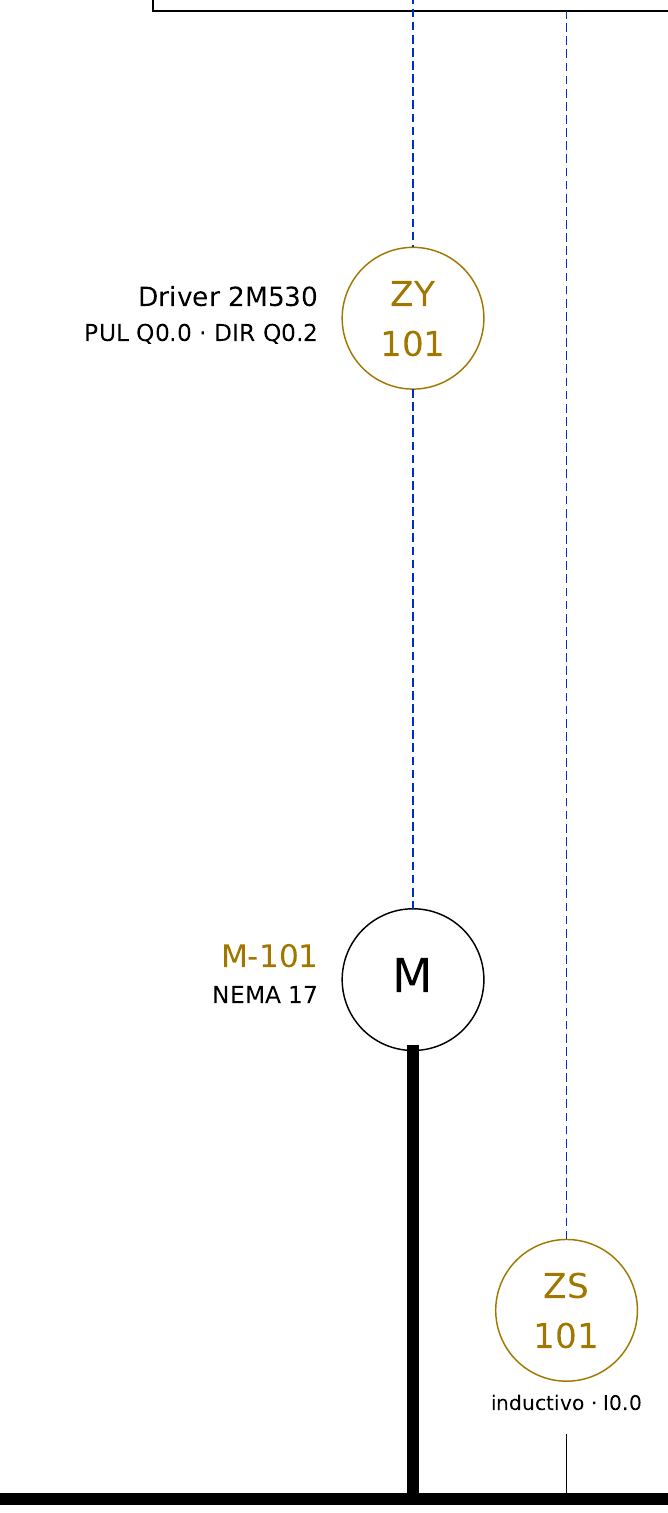
\includegraphics[width=0.54\linewidth, height=8.5cm, keepaspectratio]{pid_base}\end{figure}
Es el lazo más simple y sirve de modelo para los demás. De arriba hacia abajo:
\begin{enumerate}
\item \textbf{ZIC-101} (en el PLC) decide moverse y manda pulsos por \textbf{Q0.0} y el sentido por \textbf{Q0.2}.
\item \textbf{ZY-101}, driver 2M530: convierte cada pulso en un micropaso de corriente en las bobinas del motor.
\item \textbf{M-101}, motor paso a paso NEMA 17. La línea gruesa que baja hasta la planta es el enlace mecánico: el motor gira la base.
\item \textbf{ZS-101}, sensor inductivo (círculo simple, en campo). Detecta una marca metálica de la base y avisa al PLC por \textbf{I0.0}. Es el \emph{origen} de la base: el homing gira hasta que ZS-101 se activa y ahí pone el contador a cero.
\end{enumerate}
La línea discontinua de ZS-101 sube hasta el PLC: es la única ``realimentación'' del lazo, y solo es un punto (estoy o no estoy en el origen). No hay medida continua de la posición.

\subsection{Lazos 102 y 103: carros X e Y con el tren compartido \zona{C2--F4}}
\fig[0.8\linewidth]{pid_xy}{Lazos 102 (X) y 103 (Y). El recuadro rojo marca el nodo donde el tren de pulsos ZY-100 (Q0.1) se reparte hacia los relés K1 y K2.}
Los dos carros tienen la misma estructura que la base, con una diferencia: \textbf{no tienen salida de pulsos propia}.

\clave{El CPU 224 tiene solo \textbf{dos salidas de pulsos rápidos (PTO)}: Q0.0 y Q0.1. Hay tres motores. La solución del tablero es dar Q0.0 a la base y \textbf{repartir Q0.1 entre X e Y con dos relés}: K1 (Q0.5) deja pasar los pulsos al driver de X y K2 (Q0.6) al driver de Y. Por eso en el P\&ID el tren ZY-100 baja desde el PLC, se abre en un nodo y llega a K1 y a K2.}

Recorrido del carro X:
\begin{enumerate}
\item ZIC-102 activa \textbf{K1} con Q0.5 y fija el sentido con \textbf{Q0.3} (0 = adelante).
\item Los pulsos de Q0.1 atraviesan el contacto de K1 y llegan al driver \textbf{ZY-102} (2M542).
\item El driver mueve el motor \textbf{M-102} (NEMA 23), y este el carro X.
\item Los finales de carrera \textbf{ZSL-102} (atrás, I0.1) y \textbf{ZSH-102} (adelante, I0.2) marcan los extremos. ZSL-102 es el origen de X.
\end{enumerate}
El carro Y es igual con K2 (Q0.6), dirección \textbf{Q0.4} (0 = arriba), driver ZY-103, motor M-103 y finales \textbf{ZSL-103} (abajo, I0.3, origen de Y) y \textbf{ZSH-103} (arriba, I0.4).

\paragraph{Consecuencias del tren compartido.}
\begin{itemize}
\item Con un solo relé cerrado se mueve un solo carro. Con los dos cerrados, \textbf{X e Y reciben exactamente los mismos pulsos}: se mueven juntos la misma cantidad de pasos, cada uno en el sentido de su propia DIR. El programa encontrado usa esto a propósito en el homing (cierra K1 y K2 y lleva los dos carros al origen a la vez).
\item No se pueden mover X e Y a la vez con \textbf{velocidades o recorridos distintos}.
\item Como el contador de pulsos de Q0.1 es uno solo, el programa tiene que repartir la cuenta entre X e Y según qué relé estaba cerrado.
\item X e Y deben tener siempre los \textbf{mismos micropasos} en los DIP de sus drivers; si no, el mismo tren daría desplazamientos distintos.
\item Los relés se conmutan con el tren detenido: un contacto mecánico conduce bien los pulsos cuando está cerrado, pero no debe abrirse ni cerrarse en medio de un tren.
\end{itemize}

\subsection{Lazo 104: la garra \zona{B5--F5}}
\begin{figure}[H]\centering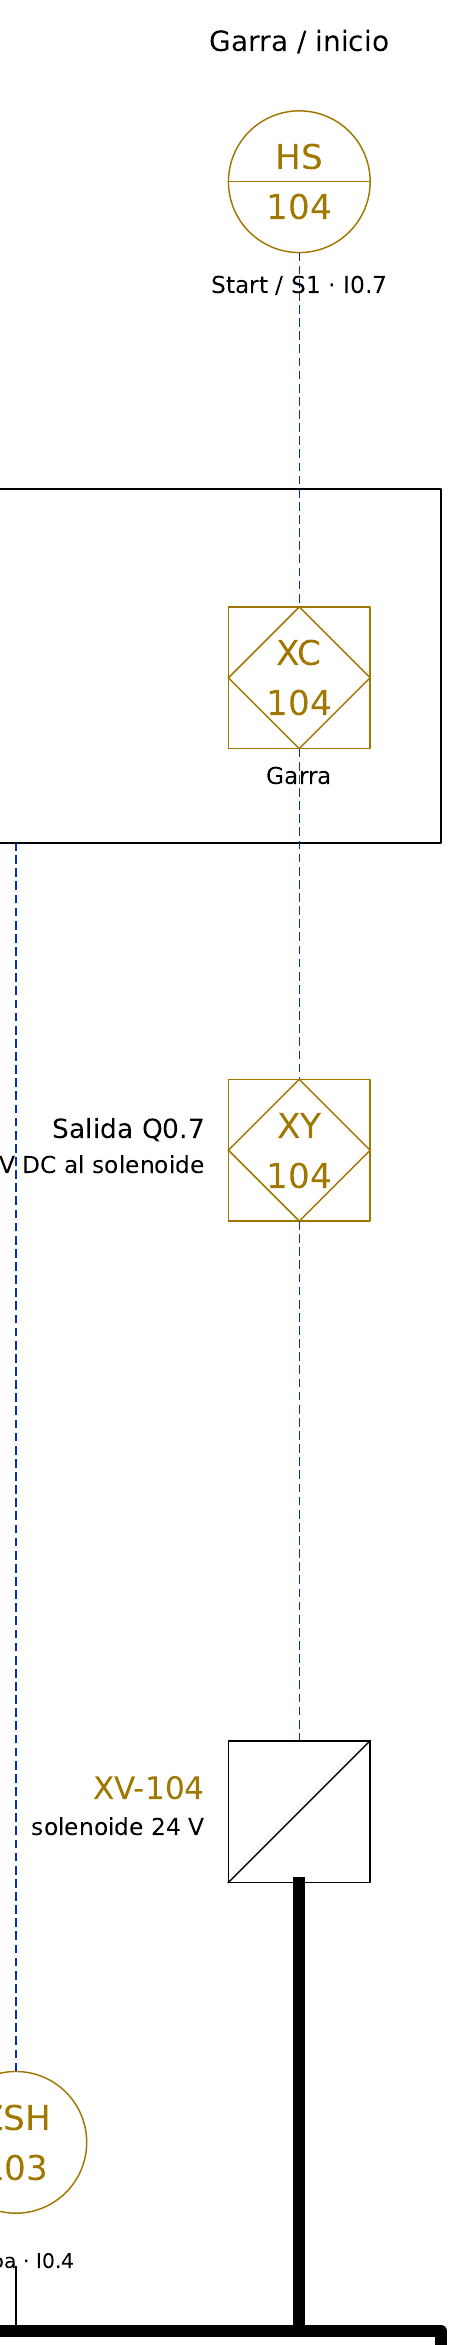
\includegraphics[width=0.36\linewidth, height=8.5cm, keepaspectratio]{pid_garra}\end{figure}
La garra no tiene motor: es un \textbf{solenoide} de 24 V.
\begin{enumerate}
\item El operador pulsa \textbf{HS-104} (Start/S1, I0.7).
\item La lógica \textbf{XC-104} del PLC cambia el estado de la garra y activa la salida \textbf{Q0.7}.
\item \textbf{XY-104} es esa salida: una función del PLC (rombo en cuadrado) que entrega 24 V DC.
\item La salida alimenta \textbf{directamente} el solenoide \textbf{XV-104} (el cuadrado con diagonal es el símbolo de actuador), que cierra la garra. No hay relé intermedio.
\end{enumerate}
No hay sensor que confirme si la garra cerró: también es lazo abierto. La letra X (sin clasificar) se usa porque la garra no mide ni controla ninguna de las variables con letra propia de la norma.

\subsection{Notas y cambios de la revisión 2.0}
\fig[0.75\linewidth]{pid_notas}{Notas del P\&ID \zona{D6}.}
\fig{pid_revision}{Recuadro rojo de la revisión 2.0 \zona{E5--E8}: lo que cambió frente al plano histórico.}
El recuadro rojo es obligatorio en un plano revisado: dice qué se cambió para que quien conocía el plano viejo sepa qué mirar. La sección~\ref{sec:cambios} explica cada cambio.

%======================================================================
\section{Esquema eléctrico, hoja 1: potencia}
%======================================================================
\fig{ele1_completo}{Hoja 1 completa: alimentación, barras de 24 V, los tres drivers con sus motores y la tabla DIP.}
La hoja 1 muestra la \textbf{energía}: de dónde entra, cómo se protege, cómo se transforma y cómo llega a los motores. Los colores ayudan a seguir los cables: \textcolor{rojo}{rojo} para fase o +24 V, \textcolor{azulw}{azul} para 0 V, \textcolor{verde}{verde} para señales y \textcolor{violet}{violeta} para referencias a otra hoja.

\subsection{Entrada de red, protección y fuente \zona{A1--C2}}
\begin{figure}[H]\centering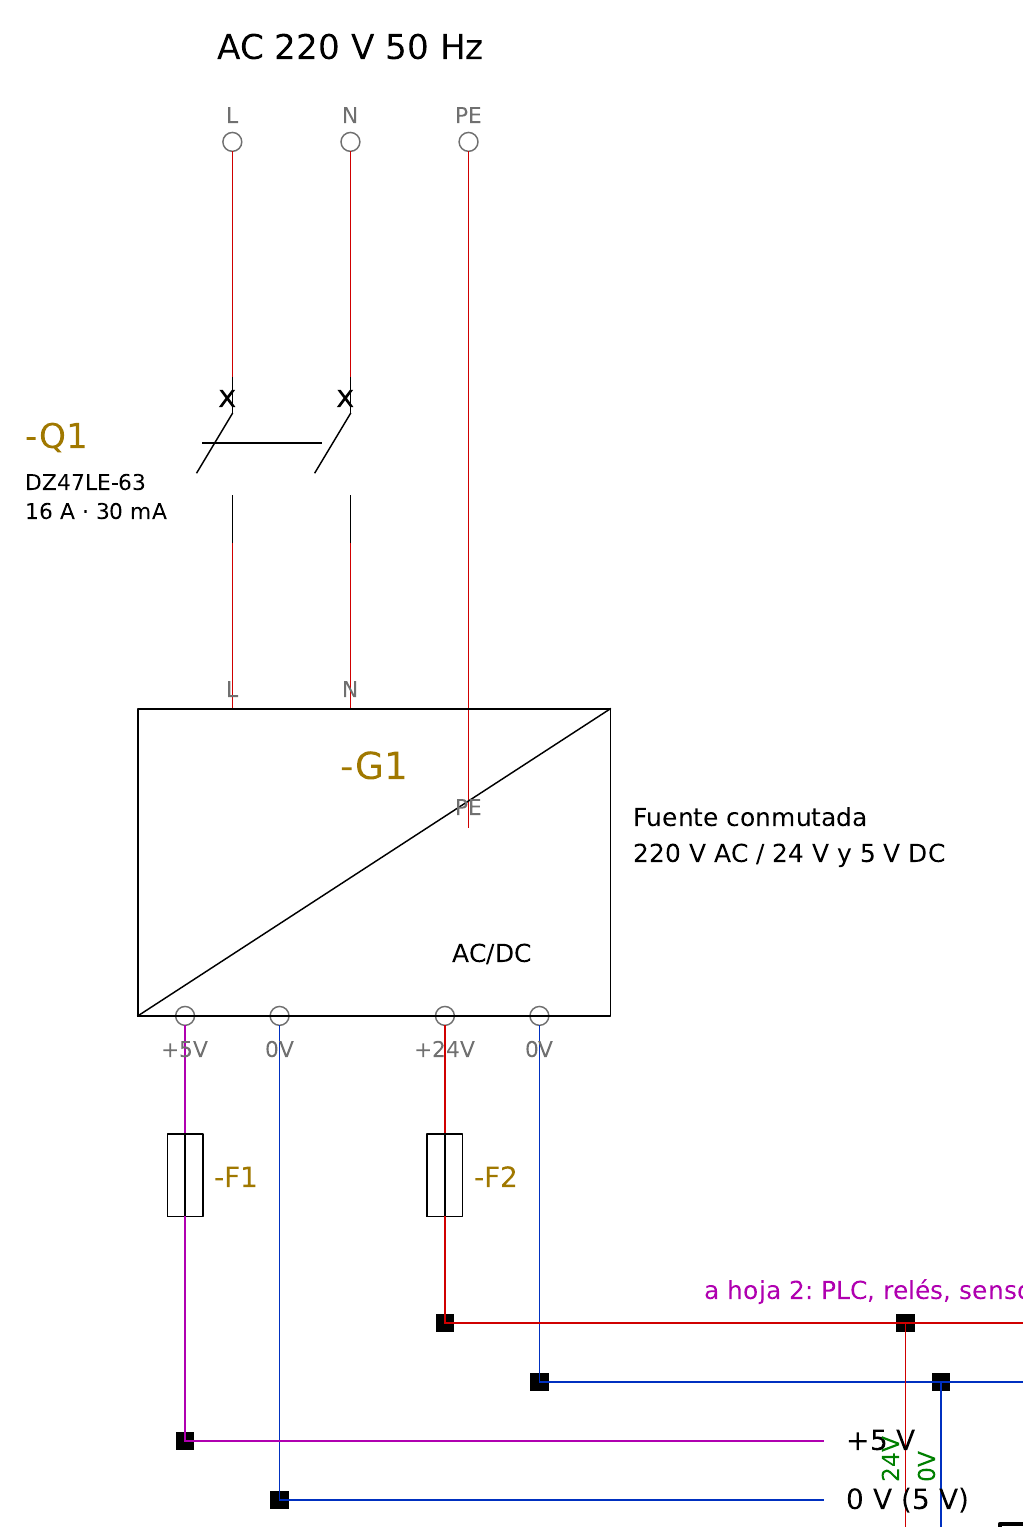
\includegraphics[width=0.72\linewidth, height=8.5cm, keepaspectratio]{ele1_alimentacion}\end{figure}
\begin{itemize}
\item \textbf{Red: 220 V AC, 50 Hz} con fase (L), neutro (N) y tierra de protección (PE).
\item \textbf{-Q1, DZ47LE-63 de 16 A y 30 mA.} Es un interruptor \emph{magnetotérmico con diferencial}. La parte magnetotérmica corta si la corriente supera 16 A (sobrecarga o cortocircuito) y protege los cables. La parte diferencial corta si hay una fuga a tierra mayor de 30 mA, que es la protección de las personas contra contacto. Por eso corta L y N (las dos cruces) pero no PE: la tierra nunca se interrumpe.
\item \textbf{-G1, fuente conmutada.} El rectángulo con una diagonal es el símbolo IEC de un convertidor (AC/DC). Convierte los 220 V AC en \textbf{24 V DC} (drivers, PLC, relés, sensores) y \textbf{5 V DC}. PE va a su carcasa.
\item \textbf{-F1 y -F2:} fusibles en las salidas de 5 V y de 24 V. Si hay un corto en el lado de continua, el fusible se abre antes de que se dañe la fuente.
\end{itemize}

\subsection{Barras de distribución \zona{C1--C8}}
\fig{ele1_barras}{Barras de +24 V (L+) y 0 V (M) que recorren la hoja; abajo a la izquierda, el par de 5 V.}
Las dos líneas largas son las \textbf{barras} de 24 V: todo lo que necesita 24 V se ``cuelga'' de ellas. Los cuadraditos negros son \textbf{puntos de conexión} (empalmes): donde hay un cuadradito, los cables están unidos; donde dos líneas se cruzan sin cuadradito, no lo están.
\begin{itemize}
\item \textbf{+24 V (L+)} y \textbf{0 V (M)}: los nombres L+ y M son los de Siemens para el positivo y la masa de 24 V. Alimentan los tres drivers y siguen a la hoja 2 (la leyenda violeta ``a hoja 2: PLC, relés, sensores (/2.1)'').
\item \textbf{+5 V y 0 V (5 V)}: par aparte para el nivel lógico de los drivers (ver~\ref{sec:opto}).
\end{itemize}

\subsection{Los drivers y los motores \zona{C2--D7}}
\fig{ele1_drivers}{Los tres drivers: -A1 (eje Y, 2M542), -A2 (eje X, 2M542) y -A3 (base, 2M530), cada uno con su motor.}
Los tres drivers se dibujan igual. Tomemos \textbf{-A1}, el del eje Y:
\fig[0.85\linewidth]{ele1_driver}{Driver -A1 (2M542) del eje Y con su motor -M1.}
\begin{itemize}
\item \textbf{V+ y GND} (izquierda, arriba): alimentación de potencia desde las barras de 24 V. De aquí sale la energía que el driver entrega al motor.
\item \textbf{A+, A-, B+, B-} (izquierda, abajo): las dos bobinas del motor paso a paso \emph{bipolar}. El driver invierte y regula la corriente en cada bobina para avanzar un micropaso por cada pulso. Si se invierten A+ y A- el motor gira al revés.
\item \textbf{PUL+ / PUL-}: entrada de pulsos. Cada pulso es un micropaso. PUL+ viene del PLC (``Q0.1 por K2 (/2.1)'': salida Q0.1, a través del relé K2, ver hoja 2 columna 1) y PUL- va a 0 V.
\item \textbf{DIR+ / DIR-}: sentido de giro. DIR+ viene de Q0.4 (/2.3); DIR- a 0 V.
\item \textbf{ENA+ / ENA-}: habilitación. Están \textbf{libres}: sin señal, el driver queda siempre habilitado y el motor retiene su posición.
\end{itemize}

\begin{center}\small
\begin{tabularx}{\linewidth}{l l >{\raggedright}X l l}
\toprule \textbf{Driver} & \textbf{Modelo} & \textbf{Motor} & \textbf{PUL+} & \textbf{DIR+}\\ \midrule
-A1 eje Y & 2M542 & -M1 NEMA 23 · 57J1854-828 · 2,8 A & Q0.1 por K2 & Q0.4\\
-A2 eje X & 2M542 & -M2 NEMA 23 · 57J1854-828 · 2,8 A & Q0.1 por K1 & Q0.3\\
-A3 base & 2M530 & -M3 NEMA 17 · 42J1848-604 · 1,2 A & Q0.0 directo & Q0.2\\
\bottomrule\end{tabularx}\end{center}

\nota{\textbf{Dos numeraciones de motores.} En el P\&ID los motores se numeran por lazo (M-101 base, M-102 X, M-103 Y); en el esquema eléctrico, por su posición en la hoja (-M1 = Y, -M2 = X, -M3 = base). Las dos son correctas en su norma. El puente entre ambas es la tabla de E/S de la hoja 2. El rótulo ``Driver eje Z (base)'' de -A3 se refiere al eje de giro de la base.}

\subsection{Cómo llega la señal del PLC a un optoacoplador}\label{sec:opto}
Las entradas PUL, DIR y ENA de los drivers son \textbf{optoacopladas}: dentro hay un LED que, al encenderse, activa un fototransistor. Así el lado del PLC y el lado de potencia del driver quedan aislados eléctricamente.

\begin{figure}[H]\centering
\begin{tikzpicture}[x=1cm,y=1cm]
\draw[hpos] (0,2) node[left, black, font=\small]{Q0.x (+24 V al activarse)} -- (1,2);
\draw[hilo] (1,2) -- (3.4,2) node[above, font=\scriptsize]{PUL+};
\draw[dashed, grisos, rounded corners] (3.2,0.4) rectangle (6.4,2.6); \node[font=\scriptsize, grisos] at (5.6,2.4){driver};
\draw[hilo] (3.4,2) -- (4,2) -- (4,1.6);
\draw[thick] (3.75,1.6) -- (4.25,1.6) -- (4,1.2) -- cycle; \draw[thick] (3.75,1.2) -- (4.25,1.2);
\draw[-{Stealth}, naranja] (4.35,1.45) -- (4.85,1.6); \draw[-{Stealth}, naranja] (4.35,1.3) -- (4.85,1.45);
\node[font=\scriptsize, align=left, right] at (4.9,1.5) {LED del\\optoacoplador};
\draw[hilo] (4,1.2) -- (4,0.8) -- (3.4,0.8) node[below, font=\scriptsize]{PUL-};
\draw[neg] (3.4,0.8) -- (0,0.8) node[left, black, font=\small]{0 V (M)};
\end{tikzpicture}
\caption{Salida del PLC hacia la entrada de pulsos de un driver.}
\end{figure}

Las salidas del S7-200 DC/DC/DC son de tipo \textbf{source} (``PNP''): al activarse entregan +24 V. Por eso PUL+ y DIR+ van a la salida del PLC y PUL- y DIR- a 0 V.

Cada pulso de la salida enciende el LED del optoacoplador y el driver avanza un micropaso; DIR funciona igual, pero se mantiene fija mientras dura el movimiento.

\subsection{Configuración DIP \zona{E1--E2}}
\fig[0.6\linewidth]{ele1_dip}{Tabla de interruptores DIP de los drivers 2M542.}
Los drivers no se programan por software: se configuran con ocho interruptores DIP. En los 2M542 de X e Y (leídos en la placa y con la tabla del fabricante):
\begin{itemize}
\item \textbf{SW1--SW3 = OFF OFF ON:} corriente de trabajo de 2,37 A pico (1,69 A RMS).
\item \textbf{SW4 = OFF:} corriente de reposo a la mitad. Cuando el motor está quieto el driver baja la corriente y el motor se calienta menos.
\item \textbf{SW5--SW8 = ON ON ON OFF:} \textbf{1000 pulsos por vuelta}. Es la cifra para convertir pulsos en vueltas del motor: 1000 pulsos = una vuelta.
\end{itemize}
El driver 2M530 de la base tiene los DIP en la misma posición que los 2M542.

\subsection{Cambios de la revisión 2.0 en la hoja 1}
\fig{ele1_revision}{Recuadro de la revisión 2.0 de la hoja 1.}

%======================================================================
\section{Esquema eléctrico, hoja 2: mando con el PLC}
%======================================================================
\fig{ele2_completo}{Hoja 2 completa: salidas del PLC arriba, el PLC en el centro, entradas abajo, la garra a la derecha y la tabla de E/S arriba a la derecha.}
La hoja 2 muestra el \textbf{mando}: qué cable sale de cada borne del PLC y qué cable entra. Las barras de +24 V y 0 V llegan desde la hoja 1 (``de /1.2'').

\subsection{El PLC -A4 \zona{B1--C5}}
\fig{ele2_plc}{El PLC con sus bornes de salida arriba y de entrada abajo.}
\textbf{Siemens S7-200 CPU 224 CN DC/DC/DC}, referencia 6ES7 214-1AD23-0XB8: 14 entradas y 10 salidas de 24 V DC, y un puerto RS-485 (puerto 0, protocolo PPI). DC/DC/DC significa que la alimentación, las entradas y las salidas son de continua (salidas a transistor, que es lo que permite generar pulsos rápidos).

Cada grupo de bornes tiene su común:
\begin{itemize}
\item \textbf{Salidas:} 1M / 1L+ alimentan el primer grupo (Q0.0--Q0.4) y 2M / 2L+ el segundo (Q0.5--Q1.1).
\item \textbf{Entradas:} 1M es el común de I0.0--I0.7 y 2M el de I1.0--I1.5.
\end{itemize}

\subsection{Salidas de pulsos y dirección \zona{A1--B3}}
\begin{figure}[H]\centering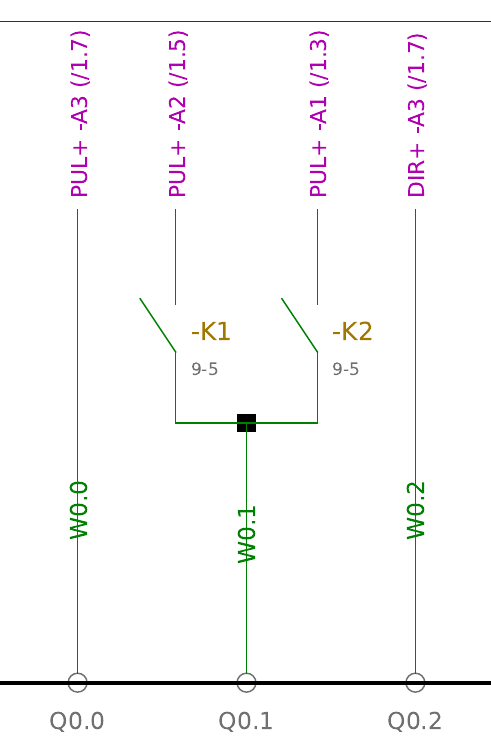
\includegraphics[width=0.45\linewidth, height=8.5cm, keepaspectratio]{ele2_pulsos}\end{figure}
Arriba de cada borne se lee hacia dónde va el cable, con referencia a la hoja 1:
\begin{itemize}
\item \textbf{Q0.0 $\rightarrow$ PUL+ de -A3} (/1.7): pulsos de la base, directo.
\item \textbf{Q0.1 $\rightarrow$ contactos 9-5 de -K1 y -K2}: el cable se abre en un empalme (cuadradito) y llega a los dos contactos. Del contacto de K1 sale \textbf{PUL+ de -A2} (X, /1.5) y del de K2 \textbf{PUL+ de -A1} (Y, /1.3). Es el tren compartido del P\&ID, dibujado como cableado real.
\item \textbf{Q0.2, Q0.3, Q0.4 $\rightarrow$ DIR+} de -A3 (base), -A2 (X) y -A1 (Y).
\end{itemize}
Los textos verdes verticales como \textbf{W0.1} son \textbf{números de hilo}: la marca que lleva cada cable en el tablero (W para los cables de salida, E para los de entrada, con el número de su borne). Sirven para encontrar el cable físico.

\subsection{Bobinas de los relés K1 y K2 \zona{A3--B4}}
\fig[0.7\linewidth]{ele2_reles}{Bobinas de los relés Omron MY2N-J en Q0.5 y Q0.6, y la salida Q0.7 hacia el solenoide de la garra.}
\begin{itemize}
\item Q0.5 y Q0.6 alimentan la \textbf{bobina} de un relé (rectángulo), entre los bornes A1 (salida del PLC) y A2 (0 V). El tablero tiene solo estos dos relés.
\item Los relés son \textbf{Omron MY2N-J de 24 V DC}: bobina en los bornes 13-14 del zócalo y contacto común 9 / normalmente abierto 5.
\item Debajo de cada bobina, en violeta, está la \textbf{referencia cruzada} a su contacto: ``9-5 /2.1'' quiere decir que el contacto 9-5 de ese relé está dibujado en la hoja 2, columna 1, en el tren de pulsos.
\item Q0.7 no lleva relé: sube con la referencia ``-Y1 garra (/2.5)'' hasta el solenoide, dibujado en la columna 5.
\item Q1.0 y Q1.1 están libres.
\end{itemize}
\clave{En un esquema IEC la \textbf{bobina} y el \textbf{contacto} de un mismo relé se dibujan donde corresponde funcionalmente, aunque estén lejos en la hoja. Lo que los une es el nombre (-K1) y la referencia cruzada.}

\subsection{Circuito de la garra \zona{C5--D5}}
\begin{figure}[H]\centering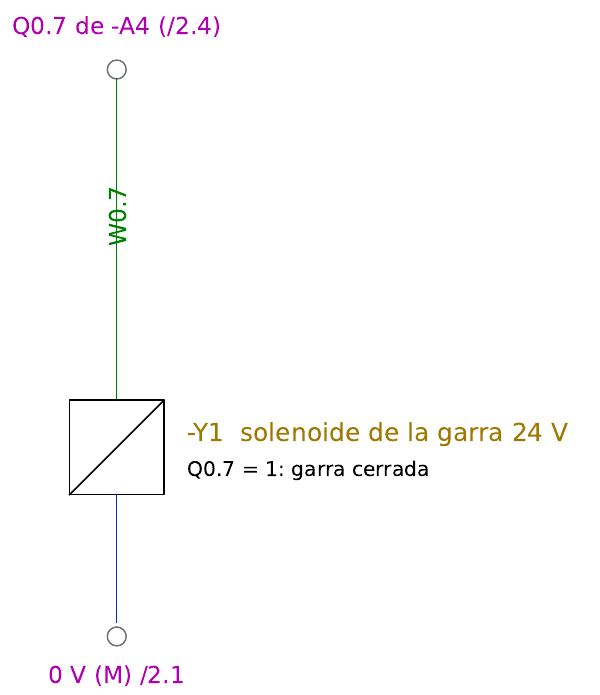
\includegraphics[width=0.54\linewidth, height=8.5cm, keepaspectratio]{ele2_garra}\end{figure}
La garra se acciona directo desde el PLC:

\textbf{Q0.7 (24 V DC) $\rightarrow$ -Y1 (solenoide de 24 V) $\rightarrow$ 0 V.}
\begin{itemize}
\item Q0.7 = 1: la salida entrega 24 V, la bobina del solenoide se energiza y la garra se cierra.
\item Q0.7 = 0: la bobina se desenergiza y la garra se abre.
\end{itemize}
La salida a transistor del S7-200 admite hasta 0,75~A por punto. El plano histórico dibujaba la bobina del solenoide con el símbolo de un relé y la llamaba ``K3''; en el tablero hay solo dos relés (K1 y K2), por eso la versión 2.0 la dibuja como lo que es: el solenoide -Y1 conectado a Q0.7.

\subsection{Entradas \zona{C1--E5}}
\fig{ele2_entradas}{Entradas del PLC: sensor inductivo, finales de carrera y botonera, todos entre su entrada y 0 V.}
\paragraph{Cómo están cableadas.} Los comunes \textbf{1M y 2M} van a \textbf{+24 V}, y cada contacto o sensor está entre su entrada y \textbf{0 V}. Así, una entrada se activa cuando su contacto la conecta a 0 V y circula corriente desde el común hacia la entrada.

\begin{figure}[H]\centering
\begin{tikzpicture}[x=1cm,y=1cm]
\draw[hpos] (-0.5,3) node[left, black, font=\small]{+24 V (L+)} -- (1.8,3) -- (1.8,2.4);
\draw[-{Stealth}, naranja, thick] (0,3.25) -- (1.2,3.25) node[right, font=\scriptsize]{corriente};
\draw[thick, fill=naranja!8] (1,-0.2) rectangle (6,2.4); \node[font=\small\bfseries] at (5.2,2.05) {PLC};
\draw[thick, fill=white] (1.8,2.4) circle (0.09); \node[font=\scriptsize, right] at (1.9,2.15) {1M};
\draw[thick] (1.8,2.31) -- (1.8,1.0) -- (2.4,1.0);
\draw[thick, fill=white] (2.4,0.6) rectangle (4.6,1.4); \node[font=\scriptsize, align=center] at (3.5,1.0) {optoacoplador\\de entrada};
\draw[thick] (4.6,1.0) -- (5.2,1.0) -- (5.2,-0.11);
\draw[thick, fill=white] (5.2,-0.2) circle (0.09); \node[font=\scriptsize, right] at (5.3,0.05) {Ix.y};
\draw[sen] (5.2,-0.29) -- (5.2,-1) -- (7,-1);
\draw[thick] (7,-1) -- (7.7,-0.65); \draw[thick] (7.8,-1) -- (8.3,-1);
\node[font=\scriptsize, above] at (7.5,-0.55) {contacto o sensor NPN};
\draw[neg] (8.3,-1) -- (9.5,-1) node[right, black, font=\small]{0 V (M)};
\end{tikzpicture}
\caption{Entrada del S7-200 con el común a +24 V: el contacto cierra hacia 0 V.}
\end{figure}

\paragraph{Por qué así: el sensor NPN de la base.}
\begin{figure}[H]\centering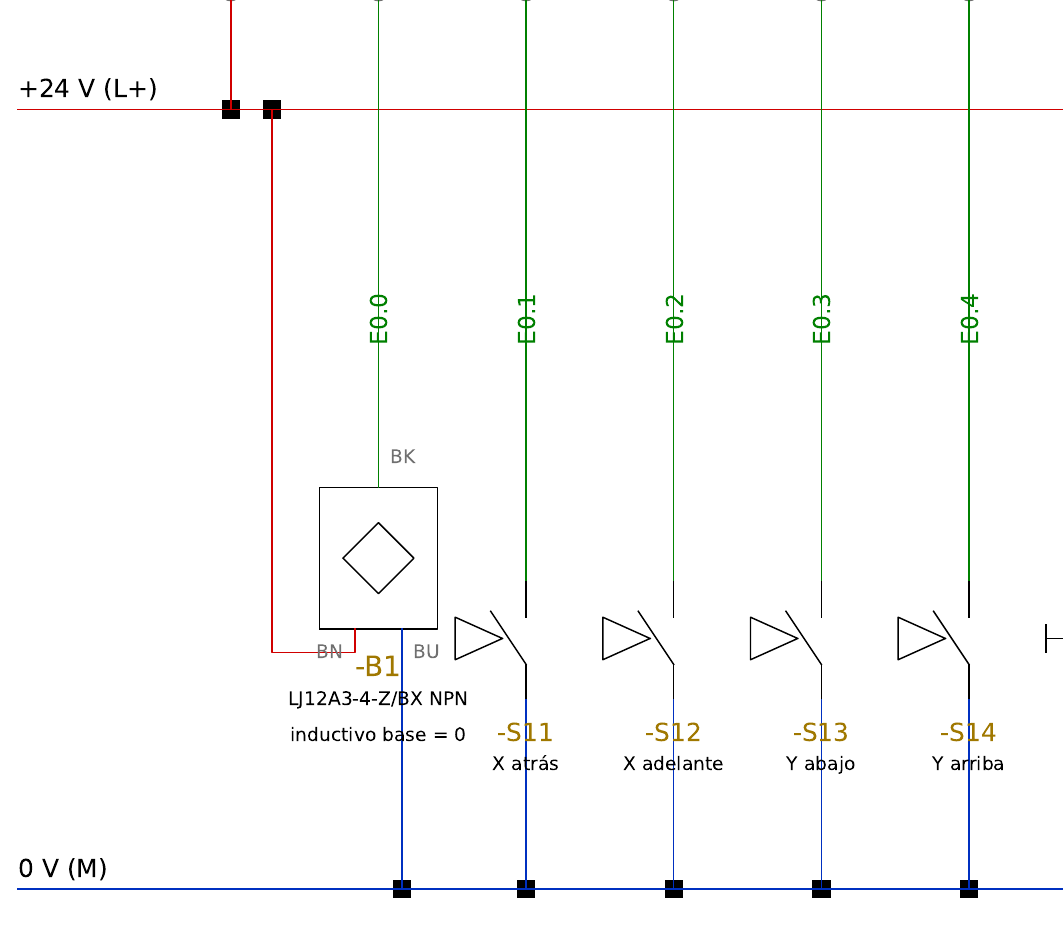
\includegraphics[width=0.68\linewidth, height=8.5cm, keepaspectratio]{ele2_sensor}\end{figure}
El sensor \textbf{-B1, LJ12A3-4-Z/BX}, es inductivo y de tipo \textbf{NPN}. Tiene tres cables:
\begin{itemize}
\item \textbf{BN} (marrón) a +24 V;
\item \textbf{BU} (azul) a 0 V;
\item \textbf{BK} (negro), la señal, a I0.0.
\end{itemize}
Un sensor NPN, al detectar, \emph{conecta su salida a 0 V}. Para que eso active una entrada, el común de esa entrada tiene que estar a +24 V. Los finales de carrera y los pulsadores están cableados con el mismo criterio, así todo el grupo es coherente.

\aviso{Según la tabla de E/S, ``inductivo base = 0'': cuando el sensor ve la marca del origen, el PLC lee \textbf{0} en I0.0. El homing de la base tiene que buscar el flanco a 0, no a 1.}

\paragraph{Qué hay en cada entrada.}
\begin{itemize}
\item \textbf{-S11 a -S14} (finales de carrera, con el símbolo de contacto accionado por leva): X atrás, X adelante, Y abajo e Y arriba, en I0.1 a I0.4.
\item \textbf{-CA}: selector manual/automático, I0.5.
\item \textbf{Reset}: paro, I0.6.
\item \textbf{Start $\parallel$ S1} en I0.7 y \textbf{Stop $\parallel$ S2} en I1.0: dos pulsadores en paralelo en la misma entrada (cualquiera de los dos la activa).
\item \textbf{S3 a S7}: jog base $-$, X+, X$-$, Y+ e Y$-$, en I1.1 a I1.5.
\end{itemize}
\begin{figure}[H]\centering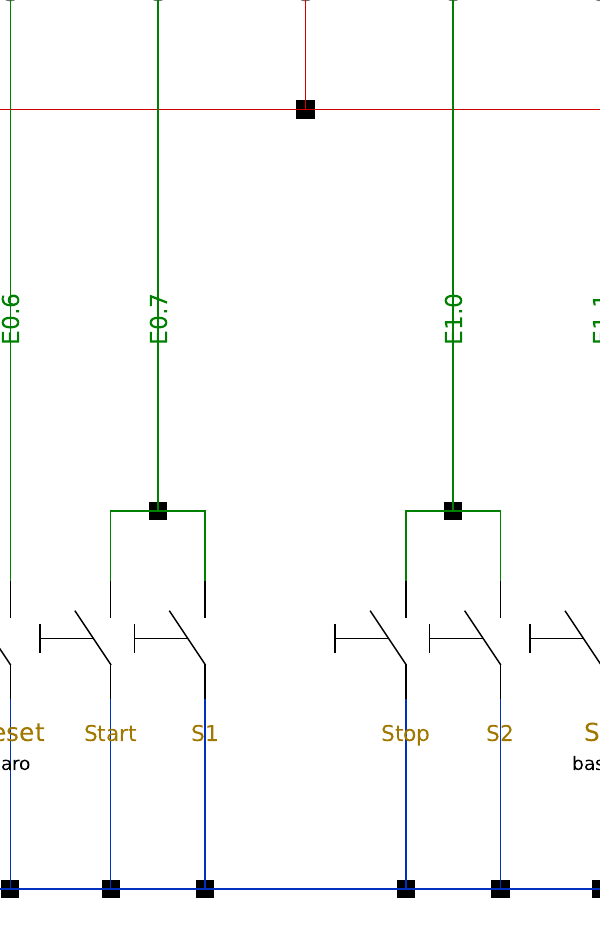
\includegraphics[width=0.54\linewidth, height=8.5cm, keepaspectratio]{ele2_paralelos}\end{figure}
\paragraph{Los paralelos.} En el recorte de arriba se ven Start y S1 unidos arriba y abajo: es una conexión en paralelo. Esto es lo que en el P\&ID aparece como ``doble función'' de los botones. Para el PLC es una sola entrada; el programa decide qué hacer según el modo (I0.5).

\subsection{Tabla de E/S \zona{A6--B8}}
\fig[0.8\linewidth]{ele2_tabla}{Tabla de entradas y salidas con su tag ISA-5.1.}
La tabla une los dos planos: para cada dirección del PLC da el \textbf{tag del P\&ID} y su función. Por ejemplo, I0.1 es ZSL-102 (final X atrás, origen) y Q0.5 es ZY-102K (K1: tren al driver X). Es la tabla que hay que tener a mano al programar el PLC o al configurar el gemelo digital.

\subsection{Notas al pie y cambios de la revisión 2.0}
\fig[0.75\linewidth]{ele2_notas}{Notas de cableado de la hoja 2.}
\fig{ele2_revision}{Recuadro de la revisión 2.0 de la hoja 2.}

%======================================================================
\section{Ejemplo completo: el operador mueve el carro X hacia adelante}
%======================================================================
Para comprobar que se entienden los planos, conviene seguir una orden por los tres planos a la vez.

\begin{center}\small
\begin{tabularx}{\linewidth}{c >{\raggedright}X >{\raggedright}p{3.2cm} >{\raggedright\arraybackslash}p{3.4cm}}
\toprule \textbf{Paso} & \textbf{Qué pasa} & \textbf{En el P\&ID} & \textbf{En el eléctrico}\\ \midrule
1 & El selector está en manual & HS-100 (I0.5) & -CA en I0.5 · hoja 2 \zona{D3}\\
2 & El operador pulsa S4 (jog X adelante) & HS-102A & S4 cierra I1.2 a 0 V · hoja 2 \zona{E4}\\
3 & El programa decide mover X & ZIC-102 & dentro del PLC -A4\\
4 & Fija el sentido adelante & — & Q0.3 = 0 $\rightarrow$ DIR+ de -A2 · hoja 2 \zona{A2}, hoja 1 \zona{D5}\\
5 & Cierra el relé de X & K1 (Q0.5) & bobina -K1 · hoja 2 \zona{B4}\\
6 & Manda pulsos & ZY-100 (Q0.1) & Q0.1 $\rightarrow$ contacto K1 9-5 $\rightarrow$ PUL+ de -A2 · hoja 2 \zona{B2}\\
7 & El driver mueve el motor & ZY-102 $\rightarrow$ M-102 & -A2 2M542 $\rightarrow$ -M2 · hoja 1 \zona{D4}\\
8 & El carro avanza (1000 pulsos = 1 vuelta del motor) & enlace grueso al carro X & —\\
9 & Llega al extremo & ZSH-102 (I0.2) & -S12 cierra I0.2 · hoja 2 \zona{E2}\\
10 & El PLC corta los pulsos y abre K1 & ZIC-102 & Q0.1 y Q0.5 a 0\\
\bottomrule\end{tabularx}\end{center}

%======================================================================
\section{Qué se corrigió frente a los planos históricos}\label{sec:cambios}
%======================================================================
Los planos históricos estaban incompletos y en algunos puntos no coincidían con el tablero. La versión 2.0 corrige:
\begin{enumerate}
\item \textbf{Entradas verificadas con el PLC en marcha.} I0.0 es el inductivo de la base; I0.1 a I0.4 son los finales X atrás, X adelante, Y abajo e Y arriba.
\item \textbf{Tren de pulsos compartido.} El histórico no explicaba cómo una sola salida Q0.1 movía dos ejes; ahora se dibujan K1 y K2 en el camino de los pulsos.
\item \textbf{Direcciones de X e Y.} Q0.3 y Q0.4 figuraban sin conexión; ahora van a DIR+ de cada driver.
\item \textbf{Garra.} El ``K3'' del histórico era la bobina del solenoide dibujada como relé; ahora Q0.7 acciona directo el solenoide -Y1.
\item \textbf{Botones en paralelo.} Start $\parallel$ S1 y Stop $\parallel$ S2 dibujados.
\item \textbf{Normalización.} Tags ISA-5.1 por lazo (100 a 104), símbolos IEC 60617, referencias cruzadas, números de hilo y tabla de E/S.
\item \textbf{Enlace al gemelo digital.} La comunicación PPI con la PC aparece en el P\&ID (ZI-100).
\end{enumerate}

\section{Mejoras propuestas para la fase siguiente}\label{sec:mejoras}
\begin{itemize}
\item \textbf{Enclavamiento eléctrico de K1 y K2.} Hoy solo el programa decide si se cierran uno, otro o los dos. Un contacto normalmente cerrado de cada relé en serie con la bobina del otro impediría que se cierren juntos por error; habría que dejar un puente o una salida aparte para el homing conjunto.
\item \textbf{Paro de emergencia cableado.} HS-100P es una entrada del PLC: el paro depende del programa. La norma IEC 60204-1 pide que la parada de emergencia corte la potencia por hardware (por ejemplo, los 24 V de los drivers o sus entradas ENA).
\item \textbf{Usar ENA.} Llevar ENA a una salida libre (Q1.0 o Q1.1) permite liberar los motores por programa.
\item \textbf{Realimentación de posición.} Un encoder por eje cerraría el lazo y detectaría pasos perdidos.
\item \textbf{Diodo de rueda libre en la garra.} Un diodo en antiparalelo con la bobina del solenoide descarga la energía de la bobina al apagar Q0.7 y alivia la salida del PLC.
\end{itemize}

\vfill
\nota{\small Planos fuente:\\ \codigo{documentacion/planos\_isa/pid/brazo\_pid\_v2.pdf}\\ \codigo{documentacion/planos\_isa/electrico/brazo\_electrico\_v2.pdf}.\\ Las imágenes de esta guía son recortes de esos PDF generados por \codigo{recortes.py}.}
\end{document}
